\section{RISE}

Like LIME, RISE\cite{Petsiuk2018rise} is a block box method and works on manipulation of the input images.

Instead of using superpixels, RISE generates masks that are then applied to the input images by multiplying the mask with the input image pixel values. Figure \ref{rise_mask0} and Figure \ref{rise_mask1} show two RISE masks applied to the same input image.

\begin{figure}[H]
    \centering
    \begin{subfigure}[t]{.32\textwidth}
        \centering
        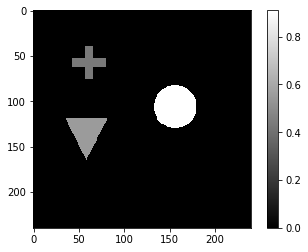
\includegraphics[width=\linewidth]{chapters/02_methods/images/rise/rise_original.png}
        \caption{Original image}
    \end{subfigure}\hfill%
    \begin{subfigure}[t]{.32\textwidth}
        \centering
        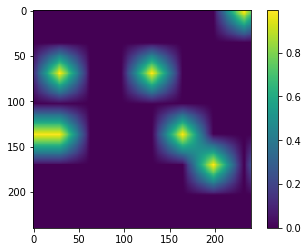
\includegraphics[width=\linewidth]{chapters/02_methods/images/rise/rise0_mask.png}
        \caption{RISE mask}
    \end{subfigure}\hfill%
    \begin{subfigure}[t]{.32\textwidth}
        \centering
        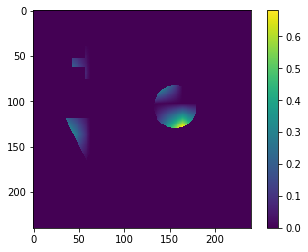
\includegraphics[width=\linewidth]{chapters/02_methods/images/rise/rise0_applied.png}
        \caption{RISE mask applied to original image by multiplication}
    \end{subfigure}
    \caption{By multiplication the input image (left) with a RISE mask (center), a modified input is generated.}
    \label{rise_mask0}
\end{figure}


\begin{figure}[H]
    \centering
    \begin{subfigure}[t]{.32\textwidth}
        \centering
        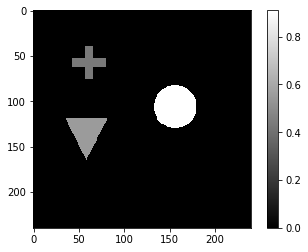
\includegraphics[width=\linewidth]{chapters/02_methods/images/rise/rise_original.png}
        \caption{Original image}
    \end{subfigure}\hfill%
    \begin{subfigure}[t]{.32\textwidth}
        \centering
        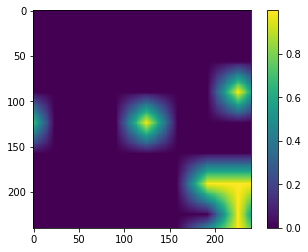
\includegraphics[width=\linewidth]{chapters/02_methods/images/rise/rise1_mask.png}
        \caption{RISE mask}
    \end{subfigure}\hfill%
    \begin{subfigure}[t]{.32\textwidth}
        \centering
        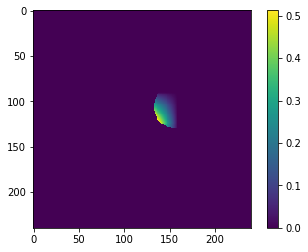
\includegraphics[width=\linewidth]{chapters/02_methods/images/rise/rise1_applied.png}
        \caption{RISE mask applied to original image by multiplication}
    \end{subfigure}
    \caption{By multiplication the input image (left) with a RISE mask (center), a modified input is generated. In comparison fo Figure \ref{rise_mask0}, this input image retains much less information.}
    \label{rise_mask1}
\end{figure}

The number of generated masks depend on the image resolution, e.g. for an image of size 240x240 pixels, 3000 masks generate good results. All masks are applied to the input image to generate new input images. The modified images are run trough the neural network and their classification scores for a specific class are recorded. A high classification score for a class on a modified input image means that the pixels preserved by the mask are important for the classification.

To visualize the results, the classific

\begin{figure}[H]
    \centering
    \begin{subfigure}[t]{\textwidth}
        \centering
        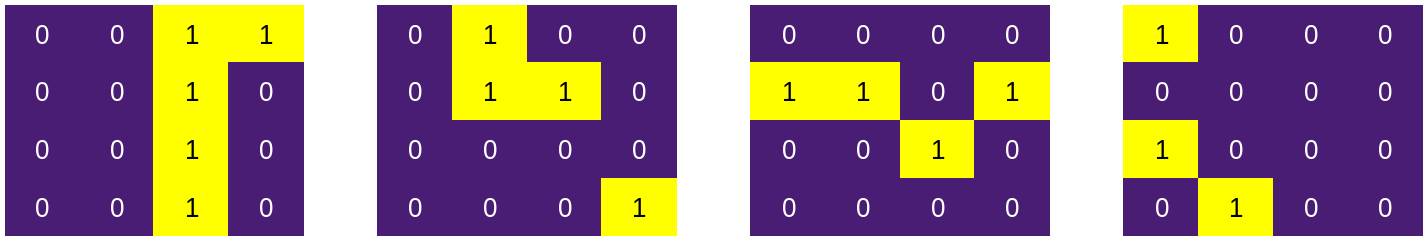
\includegraphics[width=\linewidth]{chapters/02_methods/images/rise/explain_rise_masks.png}
        \caption{Sample RISE masks}
    \end{subfigure}
    \begin{subfigure}[t]{\textwidth}
        \centering
        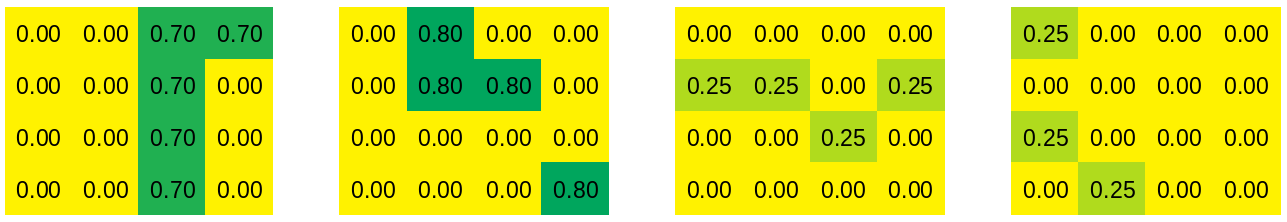
\includegraphics[width=\linewidth]{chapters/02_methods/images/rise/explain_rise_result.png}
        \caption{Masks multiplied by the classification value returned by the neural network after running the masked images trough it}
    \end{subfigure}\hfill
    \begin{subfigure}[t]{.5\textwidth}
        \centering
        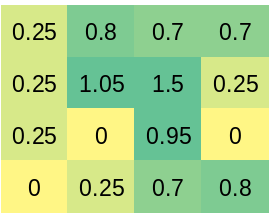
\includegraphics[width=\linewidth]{chapters/02_methods/images/rise/explain_rise_saliency.png}
        \caption{Saliency map generated by summing up all values for the same cell of the results in (b)}
    \end{subfigure}
    \caption{}
    \label{rise_explanation}
\end{figure}

To visualize the generated explanation map, the data is upscaled to the original image size and displayed as a heatmap by mapping the values to a color map. Figure \ref{rise_example} shows some examples for visualization of the RISE output for specific classes.

\begin{figure}[H]
\centering
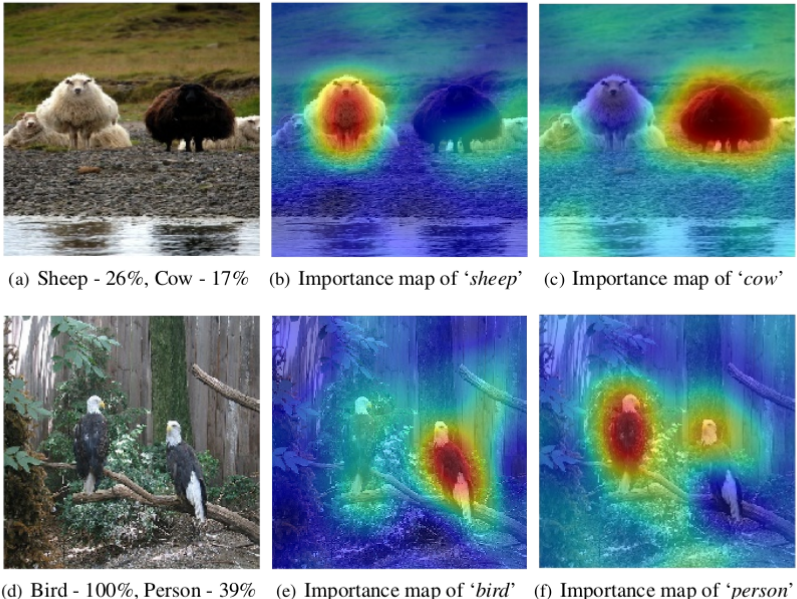
\includegraphics[width=12cm]{chapters/02_methods/images/rise/sheep.png}
\caption{Image from original paper explaining some classes}
\label{rise_example}
\end{figure}
